\documentclass[a4paper]{article}
\usepackage[latin1]{inputenc}
\usepackage{lmodern}
\usepackage[ngerman]{babel}
\usepackage{amsmath}
\usepackage{amssymb}
\usepackage{graphics}
\usepackage{graphicx}
\usepackage{cite}
\usepackage{url}

\title{Color Converter - Java Applikation zur Konvertierung zwischen Farbr\"aumen}
\author{Markus Fischb\"ock (780486)}
\date{BHT Berlin - April 2012}


\begin{document}
\maketitle
\begin{abstract}
Beschrieben ist eine Java Applikation unter Zuhilfenahme von AWT und LWJGL zur Konvertierung und Visualisierung von Farben in unterschiedlichen Farbr\"aumen.
\end{abstract}


\newpage
\tableofcontents
\newpage

\section{Einleitung}
Zu entwickeln war eine Anwendung, welche Farbwerte zwischen verschiedenen Farbr\"aumen konvertiert und
diese grafisch darstellt. Als Grundlage dieser, sollte das Java AWT Framework zum Einsatz kommen um dem
Benutzer eine grafische Oberfl\"ache zu bieten. Als Zusatz zur Anwendung sollte eine andere, als die in
der Aufgabenstellung beschriebene Visualisierung der gew"ahlten Farbe implementiert werden. Hier wurde
auf die LWJGL Library zur"uckgegriffen und eine dreidimensionale Darstellung anhand des RGB Farbraumes
gew"ahlt.\newline
Die Schwerpunkte der Aufgabe lagen darin, zum einen die Konvertierung zwischen den Farbmodellen zu
analysieren und die Implementierung mithilfe des AWT Frameworks umzusetzen.


\section{Behandelte Farbr\"aume}
Die in der Implementierung beinhalteten Farbr"aume sollen im einzelnen nun kurz vorgestellt werden.
\newline
\subsection{RGB Farbraum}
Der RGB-Farbraum beinhaltet das Farbspektrum, welches von Monitoren und Fernsehger"aten dargestellt werden
kann und erh\"alt somit besondere Bedeutung in der Computergrafik. Eine durch RGB dargestellt Farbe wird durch mischen der
einzelnen Komponenten (Rot, Gr"un, Blau) erzielt. In der hier beschriebenen Anwendung kommt dem RGB Farbraum
besondere Bedeutung zu, da zum Zwecke der Darstellung auf dem Monitor alle anderen Farben in die entsprechende RGB
Darstellung konvertiert werden.


\subsection{CMY Farbraum}
Der CMY Farbraum ist ein subtraktives Farbmodell, welches als Ausgangsfarbe schwarz verwendet. Durch
zumischen einzelner Komponenten (Cyan, Magenta, Gelb) werden andere Farben erzeugt. Das Farbmodell wird
haupts"achlich im Druck verwendet. Die Umrechnung in den RGB Farbraum gestaltet sich anhand folgender Formel:
\begin{equation}
	\label{Eq:CMY_to_RGB}
	\begin{split}
	R = 255 - C\\
	G = 255 - M\\
	B = 255 - Y
	\end{split}
\end{equation}
"Aquivalent die Umrechnung in den CMY Farbraum
\begin{equation}
	\label{Eq:RGB_to_CMY}
	\begin{split}
		C = 255 - R\\
		M = 255 - G\\
		Y = 255 - B\\
	\end{split}
\end{equation}
Quellen: (\ref{Eq:CMY_to_RGB}) und (\ref{Eq:RGB_to_CMY}) von \cite{CMYPage}\newline
Genannte Formeln sind g"ultig unter der Annahme, dass die Werte der einzelnen Komponenten im Bereich $[0;255]$ liegen.


\subsection{YUV Farbraum}
Dieser wird aus 3 Komponenten erzeugt. Dabei gibt die Y-Komponente die Helligkeit der Farbe (Luminiszenz), 
U und V werden als Chrominanz bezeichnet und geben den eigentlichen Farbanteil an. Diese k"onnen als
Vektor im $R^2$ dargestellt werden (vgl. Abbildung \ref{UVFarbspektrum}). Das Modell wurde entwickelt
um die Umstellung des Schwarz-Wei"s Fernsehens auf das Farbfernsehen zu erm"oglichen. Der Helligkeitsanteil
konnte dabei von alten Ger"aten weiterhin wie gewohnt dargestellt werden, wobei neue farbtaugliche Ger"ate
auch die zus"atzlich "ubertragenen Farbinformationen der Chrominanz ausgeben konnten. 

\begin{figure}[htp]
\centering
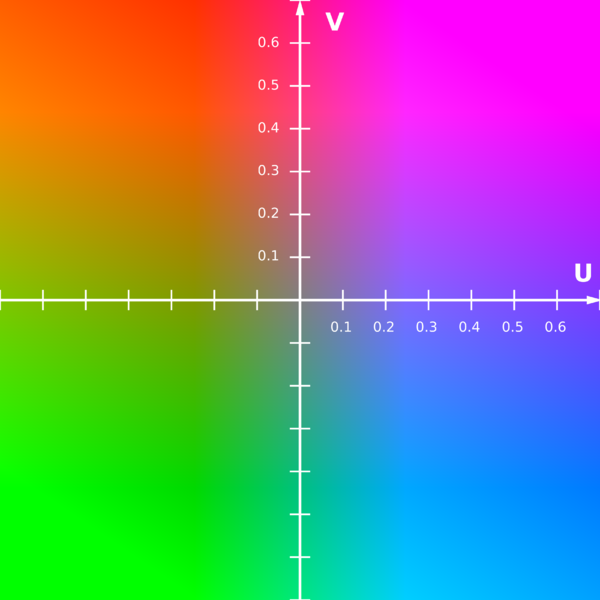
\includegraphics[scale=0.40]{600px-YUV-UV_Scaled_Y05_70_percent.png}
\caption{UV Farbspektrum}
\label{UVFarbspektrum}
\end{figure}

F"ur die Konvertierung von und in den RGB Farbraum, wurden folgende Koeffizientenmatrizen verwendet:
\begin{equation}
\label{YUV_to_RGB}
\begin{pmatrix} R \\ G \\ B\end{pmatrix} = 
\begin{pmatrix}
	1 & 0 & 1.13983 \\ 
	1 & -0.39465 & -0.58060 \\ 
	1 & 2.03211 & 0
\end{pmatrix} 
\begin{pmatrix}Y \\ U \\ V\end{pmatrix}
\end{equation}

\begin{equation}
\label{RGB_to_YUV}
\begin{pmatrix} Y \\ U \\ V\end{pmatrix} = 
\begin{pmatrix} 
	0.299 & 0.587 & 0.114 \\ 
	-0.14713 & -0.28886 & 0.436 \\
	0.615 & -0.51499 & -0.10001
\end{pmatrix}
\begin{pmatrix}R \\ G \\ B\end{pmatrix}
\end{equation}
Quellen: (\ref{YUV_to_RGB}) und (\ref{RGB_to_YUV}) von \cite{YUVPage}\newline


\subsection{HSV Farbraum}
Der HSV Farbraum wurde als zus"atzliches Farbspektrum in die Anwendung integriert. Er stellt eine Farbe
anhand dreier Komponenten dar. Dabei wird der Farbton (Hue) durch einen Gradwert angegeben, welcher die Position des
Farbtons auf einem Farbkreis wiedergibt. Durch den S"attigungswert der Farbe (Saturation) wird das Spektrum
von der "Farblosigkeit" bis hin zur Volltonfarbe verschoben. Am Beispiel der Farbe Rot mit maximaler Helligkeit sind dies anschaulich betrachtet, die Farben Wei"s und Rosa bis hin zu einem satten Rot. Durch die dritte Komponente, dem Helligkeitswert (value) kann die Farbe entsprechend aufgehellt oder abgedunkelt werden.
Zur Konvertierung von RGB nach HSV wurde im wesentlichen verwendet:

\begin{equation}
	\label{RGB_to_HSV}
	\begin{split}
	V = \max(R,G,B)\\
	m = \min(R,G,B)\\
	d = M - m\\
	\\
	S = \frac{d}{m} \cdot 255\\
	\\
	H^\prime = \begin{cases}
		\text{undefiniert}, 	& \text{f"ur}\indent d = 0\\
		\frac{G-B}{C} \mod 6, 	& \text{f"ur}\indent V = R\\
		\frac{B-R}{C} + 2, 	& \text{f"ur}\indent V = G\\
		\frac{R-G}{C} + 4, 	& \text{f"ur}\indent V = B
		\end{cases}
		\\
	H = 60^\circ \times H^\prime
	\end{split}
\end{equation}
(\ref{RGB_to_HSV}) entnommen aus: \cite{HSVPage}\newline
Zur Darstellung in der Anwendung wurde der $H$ Wert auf das Intervall $[0;255]$ umgerechnet.\newline

\section{Visualisierung anhand des RGB Farbraumes}

Um die Auswirkung einer "Anderung an einer Farbkomponente anschaulich darzustellen, wurde
in der Anwendung die Visualisierung anhand des RGB Farbraumes vorgenommen (vgl. Abbildung \ref{RGBCube}). Dazu wird mittels OpenGL
der RGB Farbraum als W"urfel im $R^3$ gezeichnet, dessen Kanten die jeweiligen Achsen R, G und B darstellen.
Innerhalb dieses Raumes markiert ein einzelner Punkt die jeweilige eingestellte Farbe. Diese Darstellung wurde
gew"ahlt, da die Auswirkung der Ver"anderung einzelner Parameter in anderen Farbsystemen gut nachvollzogen werden kann.

\begin{figure}[htp]
\centering
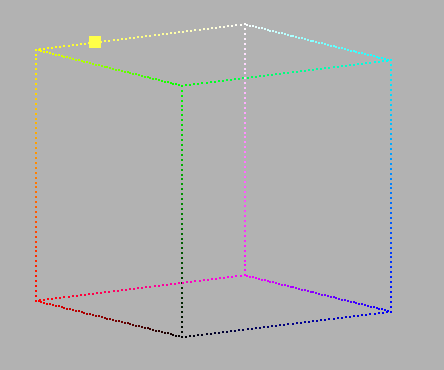
\includegraphics[scale=0.60]{RGBCube.png}
\caption{Grafische Darstellung des RGB Farbraumes}
\label{RGBCube}
\end{figure}
\newpage

\bibliography{cg-quellen.bib}{}
\bibliographystyle{gerplain}

\end{document}
